\chapter{A few example codes}

This chapter loosely presents some examples to help you get started with \LaTeX{}. You will find suggestions for implementing formulas, tables, graphs, diagrams and pseudo-code. 
In addition, there are packages for chemical structural formulas, electrical schematics, code embedding, and more, the presentation of which would go beyond the scope here.
The dummy text between the individual illustrations has as its only task to maintain a reasonable typeface despite many illustrations.

\section{Formulas}


The great strength of \LaTeX{} are formulas of all kinds. Short formulas like $b^2-4ac$ can be well placed in continuous text. Unit quantities and numbers are no problem with the \texttt{SI} package. For example, \num{6,022e23} can be represented elegantly, as can velocity in \si{\meter\per\second} or the combination of all in $a = \SI{15}{\meter\per\second\squared}$.

Extensive formulas or whole formula packages should be set in their own environment
%
\begin{align}
	a &= b + c\\
	b &= 2c + d
	\intertext{which can be easily interrupted by short text and then continued}
	a &= b + c \nonumber\\
	&= 3c + d \label{eq:eq1}
\end{align}
%
without problems. Numbering can be suppressed either line by line by \verb|\nonumber| or altogether by using the environment \verb|align*|. Of course, references, such as to \cref{eq:eq1}, are also possible.

\section{Tables, figures and plots}

\Cref{tab:tab1} shows a minimal example of a table. In contrast, \cref{tab:tab2} is already relatively complex. The start for figures is made by \cref{fig:fig0}, which is simply included here as an external image. \Cref{fig:fig1}, on the other hand, shows how to draw schemas with \texttt{TikZ} -- the template structure in \cref{fig:template_structure} on \cpageref{fig:template_structure}, by the way, is also created with \texttt{TikZ}. \Cref{fig:fig2} shows how you can plot functions with \texttt{pgfplots}, and \cref{fig:fig3} finally completes this package with the ability to read, prepare, and plot your own data, and \cref{alg:guillotine} on \cpageref{alg:guillotine} can elegantly display your pseudo-code.

\begin{table}[tb]
	\centering
	\caption{A minimal example of an elegant table.}
	\begin{tabular}{lcl}
		\toprule
		Begriff & Zeichen & Einheit\\
		\midrule
		Geschwindigkeit & $v$ & \si{\meter\per\second}\\
		Anzahl & \# & --\\
		\bottomrule
	\end{tabular}
	\label{tab:tab1}
\end{table}


\begin{table}[b]
	\centering
	\caption{A somewhat more complex, but still clear table.}
	\begin{tabular}{l@{\ }rl
			r@{\,}!{$\ldots$}@{\,}l % @{} defines horizontal spacing, !{} enables writing in column space
			r@{\,}!{$\ldots$}@{\,}l
			@{}r
		}
		\toprule
		\multicolumn{2}{l}{Parameter} & Einheit & \multicolumn{2}{c}{zulässige Menge} & \multicolumn{2}{c}{erreichtes Intervall}  & Optimum\\
		\midrule
		Durchmesser & $d_H$ & \si{\milli\metre}&\qquad\num{.1}&\num{2} &\qquad\num{.11}&\num{1.72}&\num{.811}
		\\
		\vspace{4pt}%
		Durchmesser & $d_R$ & \si{\milli\metre}&\num{.5}&\num{10}& \num{.56}&\num{9.52}& \num{.835}
		\\
		Einspritzhöhe & $h_H$ & \si{\milli\metre} &\num{25}&\num{42}& \num{25.5}&\num{41.5}&\num{36.7}
		\\
		\vspace{4pt}%
		Einspritzhöhe & $h_R$ & \si{\milli\metre} &\num{25}&\num{42}& \num{26.5}&\num{41.7}&\num{39.3}
		\\
		Einspritzwinkel & $\gamma_H$ & \si{\deg} &\num{-45}&\num{45}& \num{-42.3}&\num{41.2}&\num{14.1}
		\\
		\vspace{4pt}%
		Einspritzwinkel & $\gamma_R$ & \si{\deg} &\num{-45}&\num{45}& \num{-44.1}&\num{44.5}&\num{31.9} \\
		\bottomrule
	\end{tabular}
	\label{tab:tab2}
\end{table}

\blindtext[2]

\begin{figure}[tb]
	\centering
	
\includegraphics[width=.6\textwidth]{02_Ressources/00_Examples/LPL_Logo}
	\caption{An embedded, beautiful logo.}
	\label{fig:fig0}
\end{figure}

\begin{figure}[tb]
	\centering
	\begin{tikzpicture}[node distance = 3cm]
		
		% define some commands
		\newcommand\Foam{Open\-FOAM}
		\newcommand\Dakota{\textsc{Dakota}}
		
		% define individual styles (this can be done globally aswell)
		\tikzstyle{software} = [rectangle,  text width=3cm, rounded corners, minimum width=3cm, minimum height=1cm,text centered, draw=black, fill=gray!20, thick]
		
		\tikzstyle{steps} = [rectangle, text width=3cm, minimum width=3cm, minimum height=1cm, text centered, draw=black, fill=gray!10]
		
		\tikzstyle{main} = [diamond, text width=2cm, minimum width=2.5cm, minimum height=1cm, text centered, draw=black, very thick, fill=gray!30]
		
		\tikzstyle{arrow} = [thick,->,>=stealth]
		
		
		% define main nodes
		\node (dakota) [software] {\Dakota};
		\node (params1) [steps, right of=dakota, xshift=3cm] {Parameterdatei};
		\node[steps, below of=params1] (script) {Simulationsskript};
		\node[software, below of=script] (foam) {\Foam};
		\node[main, below of=dakota] (steuer) {\textbf{Steuer\-skript}};
		\node[steps, left of=steuer,  xshift=-3cm] (result1) {Ergebnis \Dakota-konform};
		\node[steps, below of=result1] (result2) {Ergebnis};
		%
		%
		% draw arrows
		\draw[arrow] (dakota) -- node[anchor=south] {erstellt} (params1);	
		\draw[arrow] (dakota) -- node[anchor=base east,yshift=-.1cm] {ruft auf und} node[anchor=base west,yshift=-.1cm] {übergibt Dateinamen} (steuer);	
		\draw[arrow] (result1) |- node[anchor=south west, xshift=.7cm] {wird erwartet} (dakota);
		\draw[arrow] (steuer) -- node[anchor=south,text width=2.7cm] {setzt Parameter in Vorlage ein} node[anchor=north,text width=2.7cm] {und ruft auf} (script);	
		\draw[arrow] (script) -- node[anchor=west] {startet} (foam);
		\draw[arrow] (foam) -- node[anchor=south] {liefert (ggfs. Post-Processing nötig)} (result2);	
		\draw[arrow] (result2) --  (result1);
		\draw[arrow] (steuer) -- node[anchor=south,text width=1.8cm] {formatiert Ergebnis}  (result1);
		\draw[arrow] (params1) -- (script);	
	\end{tikzpicture}
	\caption{A process schema, if you predefine the different blocks once, is relatively easy to implement with \emph{\texttt{TikZ}}.}
	\label{fig:fig1}
\end{figure}

\blindtext[2]

\begin{figure}[tb]
	\centering
	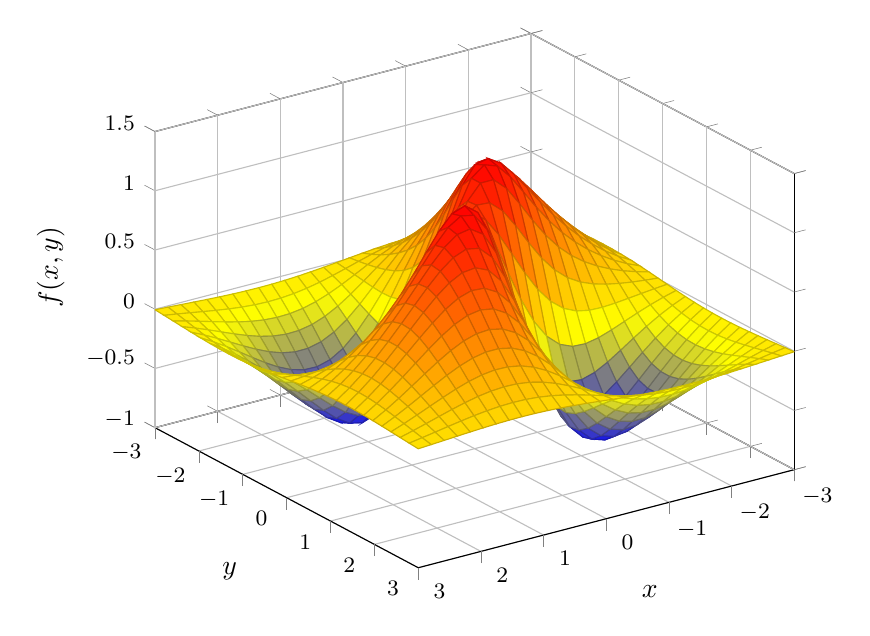
\begin{tikzpicture}% function
		\begin{axis}[
			width=.8\textwidth,
%			height={.6\textwidth},
			xlabel={$x$},
			ylabel={$y$},
			zlabel={$f(x,y)$},
			zmin=-1,
			zmax=1.5,
			xtick={-3,-2,...,3},
			ytick={-3,-2,...,3},
			ztick={-1,-.5,...,1.5},
			grid=major,
			view={145}{30},
			smooth,
			z buffer=sort,
			samples=30,
			tick align=outside,
			tick pos=left,
%			label style={font=\footnotesize},
			tick label style={font=\footnotesize},
			]
			\addplot3[
			surf,
			domain=-3:3,
			] {exp(-(x^2)-(y^2)) + (4*sin(deg(x))*sin(deg(y)) / (x^2 + y^2 + 1))};
		\end{axis}
	\end{tikzpicture}
	\caption{With the \emph{\texttt{pgfplots}} package, which is based on \emph{\texttt{TikZ}}, you can draw functions, vector fields, diagrams, etc.}
	\label{fig:fig2}
\end{figure}

\blindtext[2]

\begin{figure}[tb]
	
	% read your data (this can be done globally as well)
	\pgfplotstableread[col sep=comma]{02_Ressources/00_Examples/exampleData.csv}\exampleData
	
	\centering
	\begin{tikzpicture}
		\begin{axis}[
			width=.8\textwidth,
			height={.6\textwidth},
			xlabel = {Generation},
			ylabel = {gemittelte Mischintensität $\bar{I_S}\pm\sigma_{I_S}$},
			tick label style={font=\footnotesize},
			ylabel style={align=center},
			xmin = 0.5,
			xmax = 15.5,
			ymin = .0,
			ymax = .5,
			xtick={1,3,...,15},
			ytick distance=.1,
			tick pos=left,
			tick align=outside,
			]
			\addplot[
				restrict x to domain= 1:15,
				blue,
				mark=*,
				mark options={fill=white},
				error bars/.cd,
				y dir=both,
				y explicit,
				error bar style={thin, black},
				error mark options={thin,mark size=2pt,rotate=90},			
			] table[x={0},y={1}, y error={2}] \exampleData;
		\end{axis}
	\end{tikzpicture}

	\caption{Your raw data, for example in csv format, can be read directly with \emph{\texttt{pgfplotstable}} and then edited and plotted with \emph{\texttt{pgfplots}}.}
	\label{fig:fig3}
	
\end{figure}

\blindtext[3]

\begin{algorithm}[tb]
	\caption{You can also include pseudo code cleanly. If you want to display "real" code, on the other hand, the \emph{\texttt{lstlisting}} package is recommended.}
	\label{alg:guillotine}
	\begin{algorithmic}[1]
		\Procedure{GuillotineInsert}{Bin, item, heuristic}
		\If {$heuristic \gets best\_area$}
		\State $bestseg \gets findTheBestBestAreaScore(item)$
		\ElsIf{$heuristic \gets best\_shortside$}
		\State $bestseg \gets findTheBestBestShortsideScore(item)$
		\ElsIf{$heuristic \gets worst\_shortside$}
		\State $bestseg \gets findTheBestWorstShortsideScore(item)$
		\Else
		\State $bestseg \gets findTheBestWorstAreaScore(item)$
		\EndIf
		
		\If {$best\_rect \gets TRUE$}
		\State $Bin.addItem(item, bestseg.outline)$
		\State $Bin.freesegs.remove(bestseg)$
		\State $spliter = Bin.freeSegsSplitter(item, bestseg)$
		\For {$seg in spliter$}
		\State $Bin.freesegs.add(seg)$
		\EndFor
		\EndIf				
		\EndProcedure		
	\end{algorithmic}
\end{algorithm}

\blindtext[3]

\blindtext[2]
%\lstinputlisting[%
%	float=tb,
%	language=matlab,
%	caption={Quellcode können Sie direkt aus Ihren Programmen abrufen, oder in der \emph{\texttt{lstlisting}}-Umgebung als Pseudo-Code setzen.},
%	label=lst:lst1,
%	% weitere Anpassungen sind global in 01_Package_Setup bereits definiert
%]{02_Ressources/00_Examples/exampleCode.m}





\cleardoubleemptypage